% Created 2024-01-21 Sun 19:15
% Intended LaTeX compiler: pdflatex
\documentclass[presentation]{beamer}
\usepackage[utf8]{inputenc}
\usepackage[T1]{fontenc}
\usepackage{graphicx}
\usepackage{longtable}
\usepackage{wrapfig}
\usepackage{rotating}
\usepackage[normalem]{ulem}
\usepackage{amsmath}
\usepackage{amssymb}
\usepackage{capt-of}
\usepackage{hyperref}
\mode<beamer>{\usetheme{Madrid}}
\definecolor{SUred}{rgb}{0.59375, 0, 0.17969} % SU red (primary)
\definecolor{SUblue}{rgb}{0, 0.17578, 0.38281} % SU blue (secondary)
\setbeamercolor{palette primary}{bg=SUred,fg=white}
\setbeamercolor{palette secondary}{bg=SUblue,fg=white}
\setbeamercolor{palette tertiary}{bg=SUblue,fg=white}
\setbeamercolor{palette quaternary}{bg=SUblue,fg=white}
\setbeamercolor{structure}{fg=SUblue} % itemize, enumerate, etc
\setbeamercolor{section in toc}{fg=SUblue} % TOC sections
% Override palette coloring with secondary
\setbeamercolor{subsection in head/foot}{bg=SUblue,fg=white}
\setbeamercolor{date in head/foot}{bg=SUblue,fg=white}
\institute[SU]{Shenandoah University}
\titlegraphic{
\includegraphics[width=0.5\textwidth]{\string~/Documents/suLogo/suLogo.pdf}}
\usetheme{default}
\author{Chase Mathison\thanks{cmathiso@su.edu}}
\date{22 January 2024}
\title{Syllabus day/Review of Calc I}
\hypersetup{
 pdfauthor={Chase Mathison},
 pdftitle={Syllabus day/Review of Calc I},
 pdfkeywords={},
 pdfsubject={},
 pdfcreator={Emacs 29.1 (Org mode 9.6.7)}, 
 pdflang={English}}
\begin{document}

\maketitle

\section{Announcements}
\label{sec:org91e1d97}
\begin{frame}[label={sec:orgef11bc6}]{Announcements}
\begin{enumerate}
\item Welcome to Calc II!
\item Syllabus quiz in Canvas.
\item Homework assigned and due next Monday (mostly review).
\end{enumerate}
\end{frame}

\section{Syllabus overview}
\label{sec:org4c92abd}
\begin{frame}[label={sec:orgaa91359}]{Syllabus}
Let us take 10 minutes to review Canvas and the syllabus!
\end{frame}

\section{Calc I Review}
\label{sec:orgf8b37fd}
\begin{frame}[label={sec:org018a46d}]{Review of Calc I (Derivatives)}
Remember that Calculus I (or most of Calculus I) is about finding the
derivative, which is a generalization of the slope of a straight line.


We're going to freely use all of the rules for finding derivatives
that we developed last semester, including:


\begin{enumerate}
\item The power rule: \(\frac{d}{dx} \left( x^a \right) =\)
\item The sum/difference rule: \(\frac{d}{dx} \left( f(x) \pm g(x) \right)
   =\)
\item The product rule: \(\frac{d}{dx} \left( f(x)g(x) \right) =\)
\item The quotient rule: \(\frac{d}{dx} \left( \frac{f(x)}{g(x)} \right)
   =\)
\item The chain rule: \(\frac{d}{dx} \left( f \left( g(x) \right) \right)
   =\)
\end{enumerate}
\end{frame}

\begin{frame}[label={sec:org05dc63c}]{Review of Calc I (Derivatives)}
We'll also freely use the derivatives of elementary functions we know:


\begin{enumerate}
\item \(\frac{d}{dx} \sin (x) =\)
\item \(\frac{d}{dx} \cos (x) =\)
\item \(\frac{d}{dx} \tan (x) =\)
\item \(\frac{d}{dx} e^x =\)
\item \(\frac{d}{dx} a^x =\)
\item \(\frac{d}{dx} \ln(x) =\)
\end{enumerate}
\end{frame}

\begin{frame}[label={sec:orgc15364d}]{Reminder of the definition}
Given a function \(f(x)\) that is defined on an open interval
containing the point \(a\), we say \(f\) is differentiable at \(a\)
if

\[
\lim_{h\rightarrow 0}\hspace{2in} \]
exists. 

We call \(f'(a)\) the above limit.  If \(f\) is
differentiable at every point in an interval, we say \(f\) is
differentiable on the interval.
\end{frame}

\begin{frame}[label={sec:orgc67430b}]{Review problem}
Find the derivatives of the following functions:
\begin{enumerate}
\item \(f \left( x \right) = x^2 + 2^x\)
\item \(g \left( x \right) = e^{x^2}\)
\item \(h \left( x \right) = \frac{x^2-4}{3+2x^2}\)
\end{enumerate}
\vspace{10in}
\end{frame}

\begin{frame}[label={sec:org6eb4a8a}]{Review problem}
\end{frame}

\begin{frame}[label={sec:orga45e447}]{Review problem}
A farmer finds that if she plants 30 trees per acre, each tree will
yield 60 bushels of fruit. She estimates that for each additional tree
planted per acre, the yield of each tree will decrease by 3
bushels. How many trees should she plant per acre to maximize her
harvest?
\vspace{10in}
\end{frame}

\begin{frame}[label={sec:org7e92f56}]{Review problem}
\end{frame}

\begin{frame}[label={sec:orgad8b450}]{Review of Calc I (Integrals)}
Recall the definition of the definite integral:

\[
\int\limits_a^b f(x)\,dx = \lim_{n\rightarrow \infty}
\sum\limits_{k=1}^n f(x_k) \Delta x \]
where \(x_k = x_{0} + k\Delta x\), \(x_0 = a\), \(x_n = b\) and \(\Delta
x = (b-a)/n\).


The definite integral \(\int\limits_a^b f \left( x \right)\,dx\) is
simply the signed area under the curve defined by \(y = f \left( x
\right).\)
\end{frame}

\begin{frame}[label={sec:org699b568}]{Special note!}
The definition of the definite integral is actually more general than
what we've presented.  Really, we can define:
\[
\int\limits_a^b f(x)\,dx = \lim_{n\rightarrow \infty}
\sum\limits_{k=1}^n f(x^{*}_k) \Delta x \]
where \(x_k = x_{0} + k\Delta x\), \(x_0 = a\), \(x_n = b\) and \(\Delta
x = (b-a)/n\), and \(x_k^{*}\) is \emph{any} point in \(\left[ x_{k-1},x_k \right]\).
\vspace{10in}
\end{frame}

\begin{frame}[label={sec:orgcc02973}]{Review of Calc I (Integrals)}
We will make some use the definition of the definite integral, but
more often we will use the Fundamental theorem of Calculus:

\[
\int\limits_a^b f(x)\,dx = F(b) - F(a) \]
where \(F(x)\) is an antiderivative of \(f(x)\) on the interval
\(\left[ a,b \right]\), which means \(F'(x) = f(x)\) for each \(x\)
in \(\left[ a,b \right]\). If \(F'(x) = f(x)\) for all \(x\) in an
interval, we write
\[
\int f(x)\,dx = F(x) + C \]
\end{frame}

\begin{frame}[label={sec:org2dc75ff}]{Integration rules}
Much of this semester is going to be about finding new and better ways
to take antiderivatives to use in the fundamental theorem of calculus,
but here are a few basic rules to get us started:

\begin{enumerate}
\item \(\int x^n\,dx =\)
\item \(\int f(x) \pm g(x)\,dx =\)
\item \(\int c f(x)\,dx =\)
\item \(\int f(g(x))g'(x)\,dx =\)
\end{enumerate}

where \(F(x)\) is an antiderivative of \(f(x)\).
\end{frame}

\begin{frame}[label={sec:orgd425b01}]{Integration example}
Find
\[
\int\limits_0^3 \frac{x}{\sqrt{16+x^2}}\,dx \]
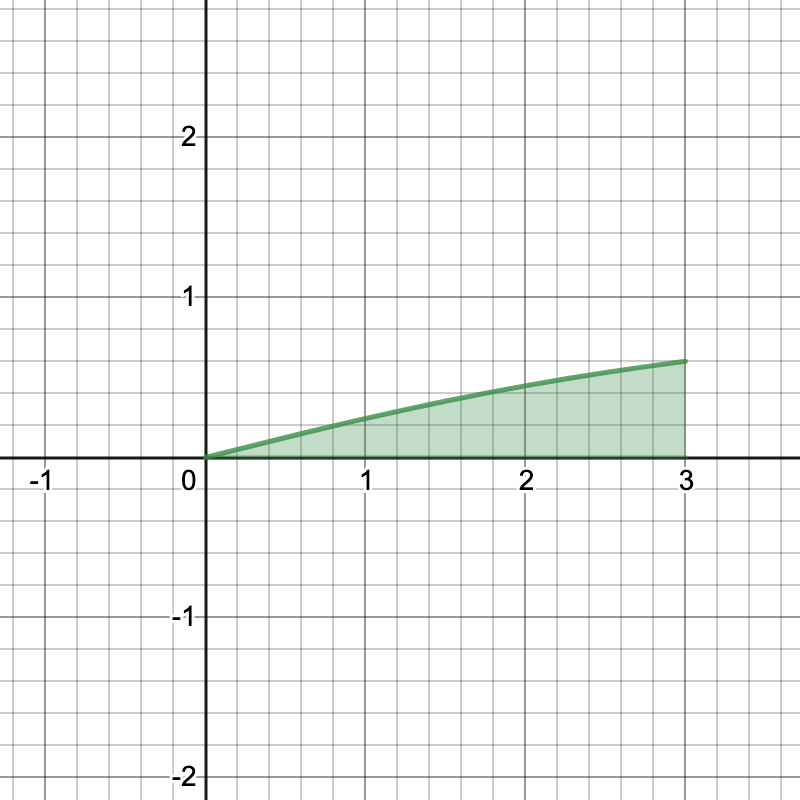
\includegraphics[width=0.5\textwidth]{../img/day001-ex2.png}
\end{frame}

\begin{frame}[label={sec:orgf2262e6}]{Integration example}
\end{frame}

\begin{frame}[label={sec:org20b1fee}]{Integration example}
Find 
\[\int\limits_0^4 \sqrt{16-x^2}\,dx \]
\vspace{10in}
\end{frame}

\begin{frame}[label={sec:orgb9b7456}]{Integration example}
\end{frame}

\begin{frame}[label={sec:org4c54ceb}]{Integration example}
Evaluate
\[
\int\limits_{-1}^1 4xe^{-10x^2}\,dx \]
\vspace{10in}
\end{frame}
\end{document}